\chapter[Multiple scales]{Introduction to the Method of Multiple Scales}

Part VIII of the course. Many of these multiple-scale techniques (and related ideas like the Poincar\'e-Lindstedt method) are conveniently illustrated on problems involving nonlinear oscillators. This is a global perturbation scheme useful in systems characterized by disparate time scales, such as weak dissipation in an oscillator. Classical perturbation methods generally break down because of resonances that lead to what are called \emph{secular}\footnote{\emph{def.} (Latin) of or denoting slow changes in the motion.} terms.

\paragraph{Example:} Duffing oscillator
\begin{gather}\label{eqn:duffing}
\frac{\md^2 y}{\md t^2} + y + \epsilon y^3 = 0, \qquad 0 < \epsilon \ll 1 \\
y(0) = 1 \qquad y'(0) = 0 \nonumber 
\end{gather}
This can be thought of as a spring problem with a weakly nonlinear restoring force 
\begin{gather*}
	F(y) = -y - \epsilon y^3
\end{gather*}
The cubic term makes it a ``hardening spring'', i.e. as the displacement $y$ increases, the restoring force becomes much stronger than that in a linear spring ($\epsilon<0$ makes it a ``softening spring''). The Duffing oscillator can be solved exactly in terms of elliptical functions, which in a way serves as a paradigmatic example for demonstrating multiple-scale analysis. Multiplying eqn. \ref{eqn:duffing} with $\md y/\md t$ we see
\begin{gather}
\frac{\md}{\md t} \left[ \frac{1}{2} \dot{y}^2 + \frac{1}{2}y^2 + \frac{1}{4} \epsilon y^4 \right] = 0 \label{eqn:wk22-duffing-energy}
\end{gather}
i.e. the quantity inside the square bracket -- total energy in fact -- is conserved (no external damping/forcing present)! Therefore the system is bounded and any admissible solution cannot grow.

\paragraph{Standard analysis: secular growth} 
Now consider the standard (regular) perturbative power-series expansion
\begin{gather}\label{eqn:perturb}
y(t,\epsilon) = y_0(t) + \epsilon y_1(t) + \epsilon^2 y_2(t) + \dots = \sum_{n=0}^{\infty} \epsilon^n y_n(t)
\end{gather}
which we assume exists with $y_0(0)=1$, $\dot y_0(0)=0$ and $y_n(0)=\dot y_n(0)=0$ for $n>0$. Substituting eqn. \ref{eqn:perturb} into eqn. \ref{eqn:duffing} and equating coefficients of like powers of $\epsilon$ up to the first two orders:
\begin{gather}
\ddot y_0 + y_0 = 0 \label{eqn:y0}\\
\ddot y_1 + y_1 = -y_0^3 \label{eqn:y1}
\end{gather}
Solution of eqn. \ref{eqn:y0} which satisfies the boundary conditions is
\begin{gather}
y_0(t) = \cos (t)
\end{gather}
which implies that we must now solve\footnote{For such problems, we want the $\cos$ and $\sin$ in harmonics and not powers. A slick way of converting them is to write $\cos t = (\me^{\mi t} + \me^{-\mi t})/2$ and cubing the exponential terms.}
\begin{gather}
\ddot y_1 + y_1 = - \frac{1}{4}\left[\cos 3 t + 3 \cos t\right] \label{eqn:y1-ode}
\end{gather}
First, we understand this \underline{heuristically}: the homogenous solution $y_h$ to the above eqn. is 
\begin{gather*}
	y_h = A \cos t + B \sin t
\end{gather*}
To determine the particular solution $y_p$, first add a driving term which is not in resonance with the natural frequency in $y_h$, so
\begin{gather*}
	y_c = y_h + C \cos 3t + \dots 
\end{gather*}
Now what happens in response to the natural frequency being driven at its resonant frequency by the $\cos t$ term on the right hand of eqn. \ref{eqn:y1-ode}? Since $\cos t$ is already part of the homogeneous term, we plug in a $t \sin t$ form. It is this term which breaks down the regular perturbative treatment as it grows unbounded.\\
\ \newline
More \underline{precisely}, we first write the solution to its homogeneous part
\begin{gather*}
y_1 = \me^{\mi t} \qquad y_2 = \me^{-\mi t} \\
W = -2\mi
\end{gather*}
The particular solution $Y_p$ is found in Python using the symbolic math module SymPy (Github repo). The constants of integration are absorbed into the homogeneous solution, which upon the application of initial conditions yield   
\begin{align}
y &\simeq y_0 + \epsilon y_1 + \cancel{\epsilon^2 y_2 + \dots} \nonumber \\
&\simeq \cos t + \epsilon \left[\frac{1}{32} \cos 3t - \frac{1}{32} \cos t - \frac{3}{8} t \sin t\right] \label{eqn:duffing-secular}
\end{align}
The $t$ dependence in $y_1$ is known as secular growth and arises whenever there is a resonance between $y_0$ and $y_1$. There are two clear issues with this treatment:
\begin{itemize}
	\item The secular term $\epsilon t \sin t$ which grows unbounded as $t \rightarrow \infty$
	\item When $t=O(1/\epsilon)$, $y_0$ and $y_1\approx \epsilon t \sin t$ become comparable, but we want $y_0 \gg \epsilon y_1$ for good asymptotics. 
\end{itemize}
So what causes the problem? Our model
\begin{gather*}
	\ddot y + (1+\epsilon y^2) y = 0
\end{gather*}
has a spring stiffness $k = 1+\epsilon y^2$. Since the spring gets stiffer with displacement, we expect its frequency to increase too (softer springs will oscillate slowly). We therefore expect the $\epsilon y^2$ term to alter the frequency cf. the $\epsilon=0$ case. But regular perturbation theory forced us to assume the frequency is given by the unperturbed frequency $(\omega=1)$. This is how the errors start accumulating. 

\paragraph{NB.} If we keep infinitely many terms ($O(\epsilon^2)$ etc) we expect to get the right solution through cancellations. But this is laborious and motivates several alternative approaches. 

\paragraph{Poincar\'e-Lindstedt method} Early (no longer state-of-art) method but is instructive and good for approximating periodic solutions, but not for analyzing transients or stability. Begin by letting
\begin{gather*}
	\tau = \omega t
\end{gather*} 
where $\omega = \omega(\epsilon)$ is a power series in $\epsilon$ :
\begin{gather*}
	\omega = \omega_0 + \epsilon \omega_1 + \epsilon^2 \omega_2 + \dots 
\end{gather*}
We will determine $\omega$ by insisting that it's the \emph{true frequency} and hence the \underline{solution is $2\pi$ periodic in $\tau$}. This converts the problem to one we can solve with regular perturbation theory:
\begin{gather*}
	\omega^2 \frac{\md^2 Y}{\md \tau^2} + Y + \epsilon Y^3 = 0 \\
	Y(0) = 1 \qquad \omega Y'(0) = 0
\end{gather*}
where $Y = y(\tau(t))$. Now using a regular perturbative expansion for $Y$
\begin{flalign*}
	(\omega_0 + \epsilon \omega_1 + \dots)^2 (Y_0'' + \epsilon Y_1'' + \dots )& \\
	+(Y_0 + \epsilon Y_1 + \dots )& \\
	+\epsilon (Y_0 + \epsilon Y_1 + \dots)&^3 = 0
\end{flalign*}
with the ICs
\begin{flalign*}
	Y_0(0) + \epsilon Y_1(0) + \dots  &= 1 \qquad \forall \epsilon \\
	(\omega_0 + \epsilon \omega_1 + \dots ) (Y_0'(0) + \epsilon Y_1'(0) + \dots ) &= 0 \qquad \forall \epsilon
\end{flalign*}
This results in the hierarchy of equations:
\begin{align*}
	O(\epsilon^0): \qquad & \omega_0^2 Y_0'' + Y_0 = 0 \\
	O(\epsilon^1): \qquad & \omega_0^2 Y_1'' + Y_1 = - Y_0^3 - 2 \omega_0 \omega_1 Y_0''
\end{align*}
The $O(1)$ equation must satisfy the ICs $Y_0(0)=1$ and $Y_0'(0)=0$, yielding
\begin{gather*}
	Y_0(\tau) = \cos \left(\frac{\tau}{\omega_0}\right)
\end{gather*}
Note that in the second IC, we required that $\omega_0 Y_0'(0)=0$. Since $\omega_0=0$ would imply that $Y_0=0$ for all time ($O(1)$ equation), violating the first IC $Y_0(0)=1$, it must be that $\omega_0 \neq 0$. \\
\ \newline
Now we impose the requirement -- taken true at every order -- that $Y_0(\tau)$ is $2\pi $ periodic in $\tau$. Since we may express periodic functions as
\begin{gather*}
	\cos \left(\frac{2\pi}{T} t\right) = \cos \left(\frac{2\pi}{T}\frac{\tau}{\omega }\right)
\end{gather*} where the time-period $T=2\pi/\omega $, this forces
\begin{gather*}
	\omega_0 = 1
\end{gather*} 
All this is saying that we have chosen $\omega$ to be the correct frequency such that $2\pi/\omega$ is the fundamental period of the oscillation. Next, the $O(\epsilon)$ equation reads
\begin{align*}
	Y_1'' + Y_1 &= - Y_0^3 - 2 \omega_1 Y_0'' \\
	&= -\frac{1}{4} \cos 3 \tau - \underbrace{\left[\frac{3}{4} - 2 \omega_1\right]}_\text{secular} \cos \tau
\end{align*}
Recall that it was this resonant term which was causing the secular growth. Here in fact we have the option of choosing $\omega_1 = 3/8$ to get rid of this term! This also predicts a frequency that varies as
\begin{gather*}
	\omega = 1 + \frac{3}{8} \epsilon + O(\epsilon^2)
\end{gather*}
We solve the ODE for $Y_1''$: 
\begin{gather*}
	y_h = A \sin \tau + B \cos \tau \\
	y_p = C \cos 3 \tau 
\end{gather*}
First determine $C$ through
\begin{gather*}
	-9C \cos 3 \tau + C \cos 3 \tau = -\frac{1}{4} \cos 3 \tau \\
	\implies C = \frac{1}{32}
\end{gather*}
Now the equation
\begin{gather*}
	Y_1(\tau) = A \sin \tau + B \cos \tau + \frac{1}{32} \cos 3 \tau 
\end{gather*}
must satisfy the ICs
\begin{gather*}
Y_1(0) = 0 \qquad Y_1'(0)\cancelto{1}{\omega_0}  \quad + \omega_1 \cancelto{0}{Y_0'(0)} = 0
\end{gather*}
yielding
\begin{gather*}
	A = 0 \qquad B = -\frac{1}{32}
\end{gather*}
Pulling it all together
\begin{align*}
	Y(\tau) &= Y_0 + \epsilon Y_1(\tau ) + O(\epsilon^2) \\
	&= \cos \tau + \epsilon \left[\frac{1}{32}\left(\cos 3 \tau - \cos \tau\right)\right] + O(\epsilon^2) 
\end{align*}
where 
\begin{gather*}
	\tau = \left(1 + \frac{3}{8}\epsilon + \dots\right) t
\end{gather*}
The first term, neglecting $O(\epsilon)$ and higher terms, are also given by eqn. \ref{eqn:duffing-analytic} and plotted in Fig. \ref{fig:duffing}. The agreement at even this order is quite excellent.
\begin{figure}[!h]
	\centering
	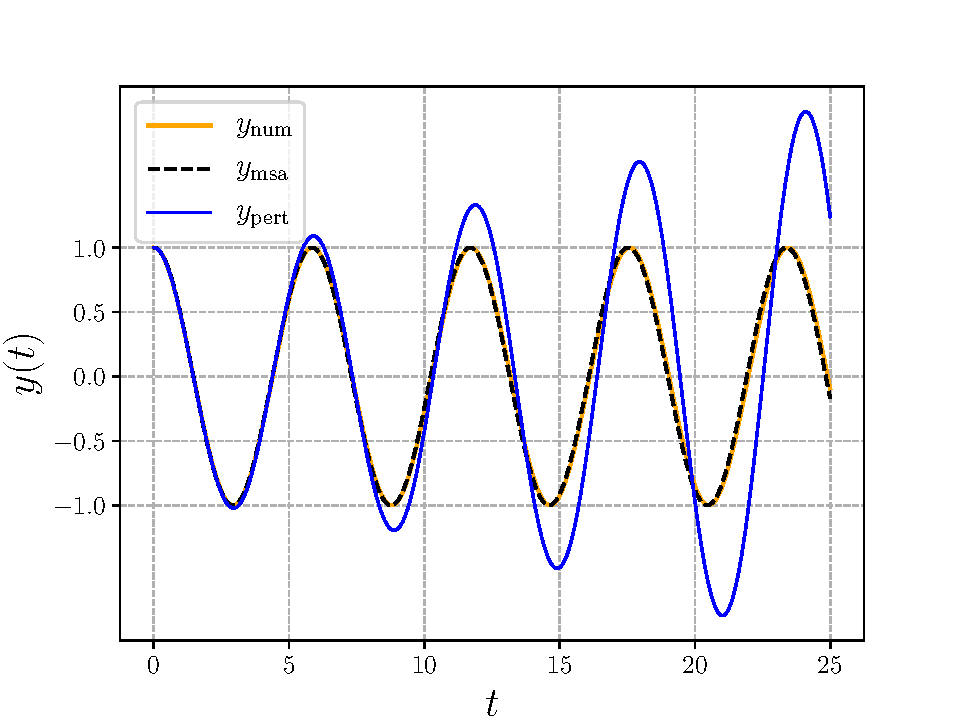
\includegraphics[width=0.7\textwidth]{./plots/pdf/strogatz-wk22-duffing.pdf}
	\caption{Plots of direct numerical solution to eqn. \ref{eqn:duffing}, simple perturbative analysis yielding eqn. \ref{eqn:duffing-secular} and solution using multi-scale analysis eqn. \ref{eqn:duffing-analytic} for $\epsilon=0.2$. }
	\label{fig:duffing}
\end{figure}